\begin{refsection}

\chapter{Th--Pb}
\label{ch:ThPb-R}

\noindent\begin{minipage}[t]{.3\linewidth}
\strut\vspace*{-\baselineskip}\newline
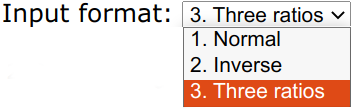
\includegraphics[width=\linewidth]{../figures/PbPbFormats.png}
\end{minipage}
\begin{minipage}[t]{.7\textwidth}
  \texttt{IsoplotR} accommodates three Pb--Pb formats. See
  Section~\ref{sec:PbPb} for details.
\end{minipage}

\begin{console}
PbPb <- read.data('PbPb.csv',method='Pb-Pb',format=3)
\end{console}

\noindent\begin{minipage}[t]{.15\linewidth}
\strut\vspace*{-\baselineskip}\newline
\includegraphics[width=\linewidth]{../figures/PbPbPlotdevices.png}\\
\end{minipage}
\begin{minipage}[t]{.85\textwidth}
  Pb--Pb data can be visualised on five different plot devices.
  Additionally, the single aliquot age estimates can also be reported
  in a downloadable data table.
\end{minipage}

\noindent\begin{minipage}[t]{.6\linewidth}
\strut\vspace*{-\baselineskip}\newline
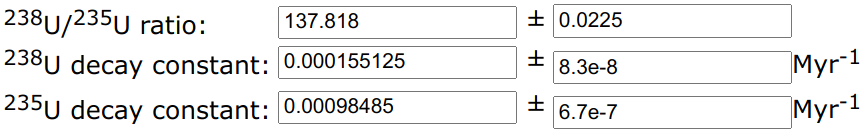
\includegraphics[width=\linewidth]{../figures/PbPbLambda.png}
\end{minipage}
\begin{minipage}[t]{.4\linewidth}
  The default \textsuperscript{238}U/\textsuperscript{235}U ratio is
  given by \citet{hiess2012}, and the U decay constants by
  \citet{jaffey1971}. These values can be changed here.
\end{minipage}

\begin{script}
# use the Steiger and Jaeger (1977) value with zero uncertainty
settings('iratio','U238U235',137.88,0)
# use the Schoene et al. (2006) value and uncertainty
settings('lambda','U238',0.000154993,0.00000013) 
\end{script}

\section{Isochrons}

\section{Radial plots}

\section{Weighted mean}

\section{Kernel density estimates}

\section{Cumulative age distributions}

\section{Ages}

\printbibliography[heading=subbibliography]

\end{refsection}
